%Correct the file name.
%X: book number
%Y: part number
%ZZZ: page number in three digits. So page 3 would be 003.

\documentclass[12pt]{amsbook}

\usepackage{../HBSuerDemir}	% ------------------------
\footnote{see/comments/at/top}
% Sayfamda iki numaralandırma var fakat ifadelere kendisine özel bi isim vermiş (1') gibi mesela. begin{align} veya begin{equation} denedim fakat işlem çok uzun olduğu için ya sayfadan taştı ya da tamamen ignore etti gibi bir şey oldu. Başa çıkamadım ve kendimce parantez açıp kapatarak özel isimlerini yazdım. Not olarak söylemek istedim. Teşekkürler.%


\begin{document}

% ++++++++++++++++++++++++++++++++++++++
\hPage{b2p1/215}
% ++++++++++++++++++++++++++++++++++++++

\begin{tabular}{c c c}
\begin{array}{lcl}
      $A_1$ & = & $a_{11}$, \\
      $B_1$ & = & $2a_{23}$, \\
      $C_1$ & = & $2a_{14}$,  
    \end{array}
    &
	\begin{array}{lcl}
      $A_2$ & = & $a_{22}$, \\
      $B_2$ & = & $2a_{31}$, \\
      $C_2$ & = & $2a_{24}$,  
    \end{array}
    &
	\begin{array}{lcl}
      $A_3$ & = & $a_{33}$, \\
      $B_3$ & = & $2a_{13}$, \\
      $C_3$ & = & $2a_{34}$ , $D =a_{44}$ 
    \end{array}
\end{tabular}
\\
\\
with $a_{ij}=a_{ji}$. Then $(1')$ becomes
\[a_{11}x_1^2 + a_{22}x_2^2 + a_{33}x_3^2\] 
\[ + 2a_{23}x_2x_3 + 2a_{31}x_3x_1 + 2a_{12}x_1x_2\]
\[ + 2a_{14}x_1x_4 + 2a_{24}x_2x_4 + 2a_{34}x_3x_4 + a_{44}x_4^2 = 0\]
or
\\
\begin{center}
\begin{tabular}{c c}
    \[a_{11}x_1^2 + a_{12}x_1x_2 + a_{13}x_1x_3 + a_{14}x_1x_4 \] \\
    \[+ a_{21}x_2x_1 + a_{22}x_2^2 + a_{23}x_2x_3 + a_{24}x_2x_4\] \\
    \[ + a_{31}x_3x_1 + a_{32}x_3x_2 + a_{33}x_3^2 + a_{34}x_3x_4\] \\
    \[+ a_{41}x_4x_1 + a_{42}x_4x_2 + a_{43}x_4x_3 + a_{44}x_4^2 = 0\]
     & 
     \\
     \[(1'')\]
     \\
\end{tabular}
\end{center}
which is seen to be the same as
\\
\[\begin{bmatrix}x_1 & x_2 & x_3 & x_4\end{bmatrix}
\begin{bmatrix}a_{11} & a_{12} & a_{13} & a_{14} \\ a_{21} & a_{22} & a_{23} & a_{24} \\ a_{31} & a_{32} & a_{33} & a_{34} \\ a_{41} & a_{42} & a_{43} & a_{44}\end{bmatrix}
\begin{bmatrix}x_1 \\ x_2 \\ x_3 \\ x_4\end{bmatrix} =0, (x_4=1)
\]
\begin{center}
\[(2)\]
\end{center}
\\
where the matrix $\begin{bmatrix}a_{ij}\end{bmatrix}$ is symmetric.
\\


When $(2)$ is written in the original notation, we have (for $x_4 =1$)

% =======================================================
\end{document}  

%==== templates ====

%==== environments ====

%\begin{figure}[htb]
%	\centering
%	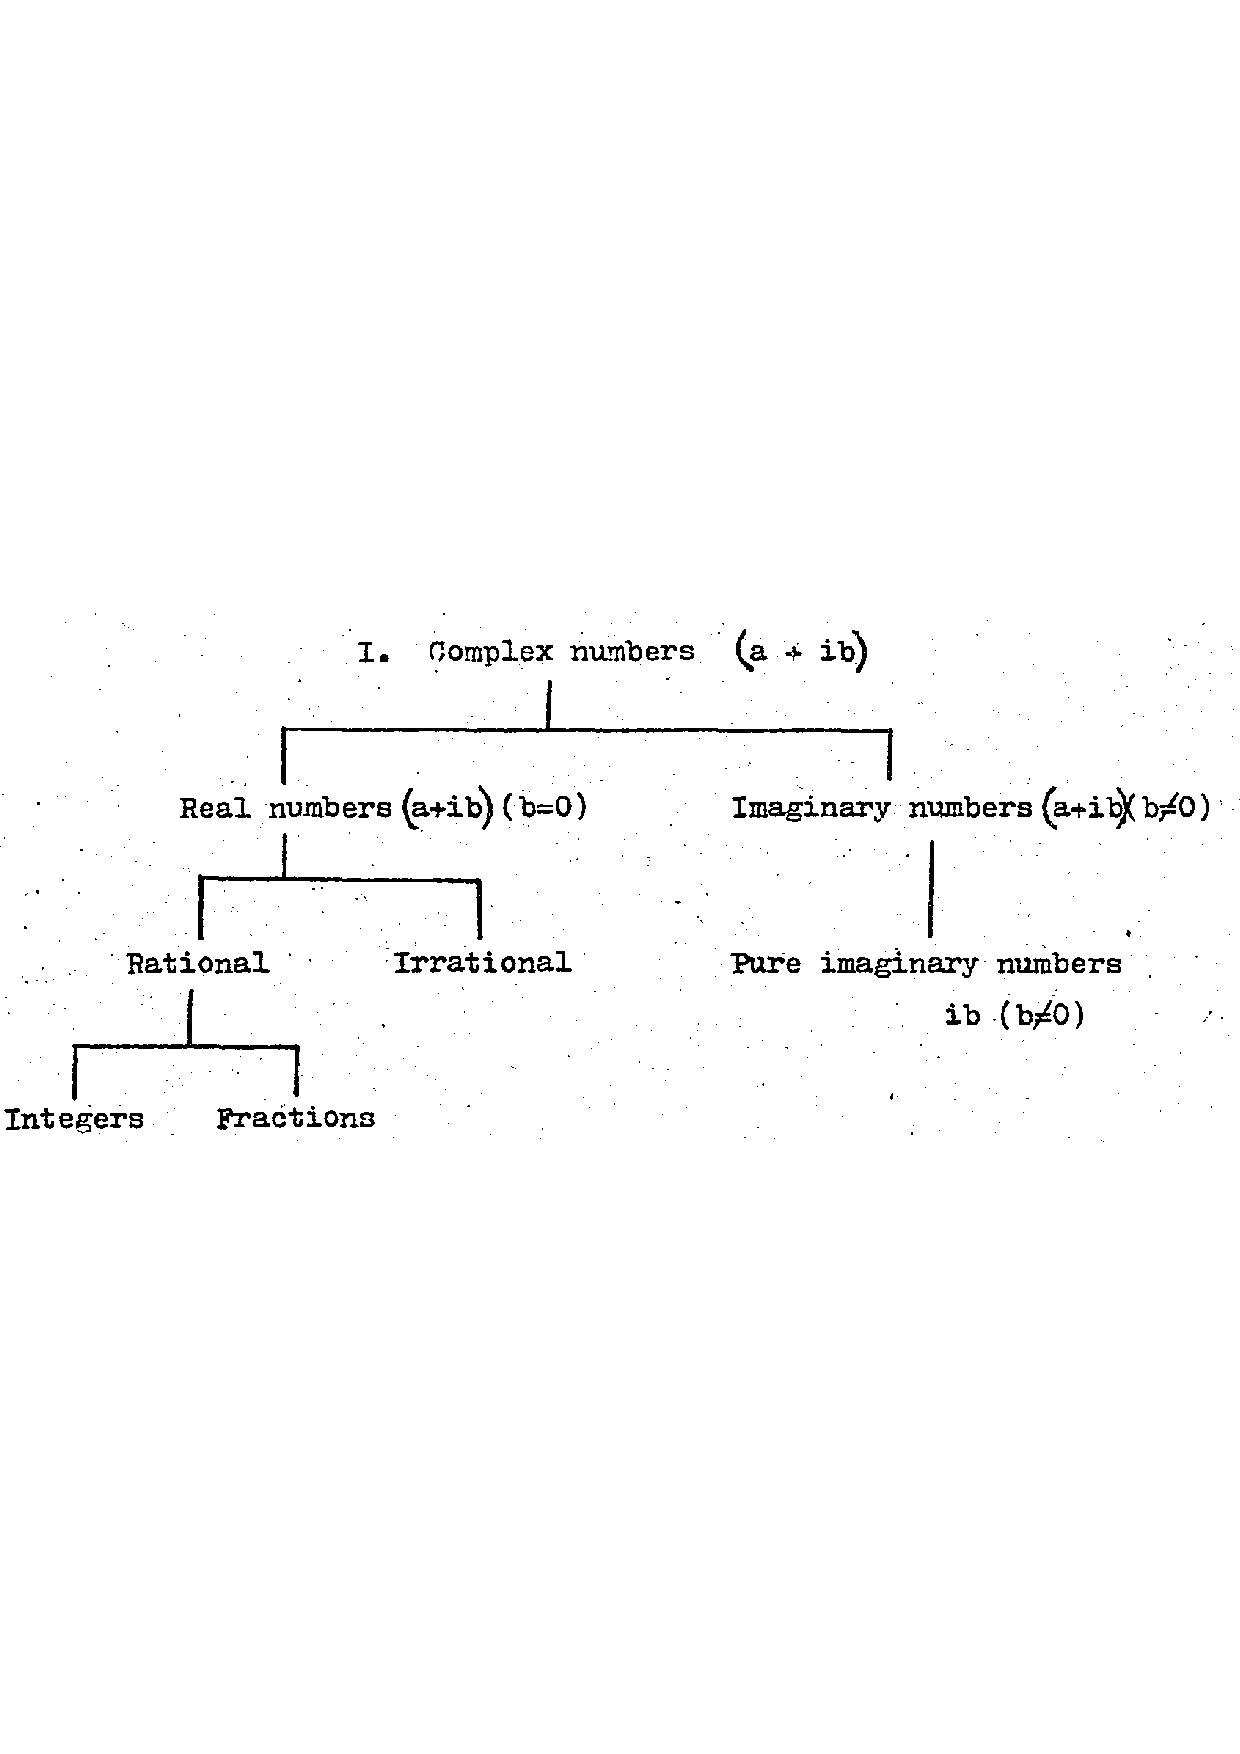
\includegraphics[width=0.9\textwidth]{images/SD-1-1p15A}
%	\caption{Classification of complex numbers}
%	\label{fig:classificationOfComplexNumbersA}
%\end{figure}

%\begin{center}
%\begin{tabular}{cc}
%\end{tabular}
%\end{center}

%\begin{exmp}
%\begin{hSolution}
%\end{hSolution}
%\end{exmp}

%\begin{hEnumerateAlpha}
%\end{hEnumerateAlpha}

%\begin{hEnumerateRoman}
%\end{hEnumerateRoman}

%$
%\begin{bmatrix}
%\end{bmatrix}
%$

%\frac{aaaa}{bbb}
%\frac{a_{n}}{b_{n}}
%\left( aaaa \right)
%\Longrightarrow

%\begin{multicols}{2}
%	bb
%\columnbreak
%	aa
%\end{multicols}
